\section{Description}
\label{part:describ}
In this part we will describe the construction of the one dimensional PML from elastodynamics wave equations to the finite elements formulation.
\subsection{Elastic medium}
In the following of this report we will consider a one dimensional homogeneous isotropic elastic continuum. In such medium the displacement $u(x,t)$ is governed by the following equations:
\begin{equation}
  \begin{aligned}
    \frac{\partial \sigma}{\partial x} &= \rho \Ddot{u}\\        
    \sigma &= E \epsilon \\
    \epsilon &= \frac{\partial u}{\partial x}
  \end{aligned}
  \label{eq:governed_equation}
\end{equation}
In the equations of \ref{eq:governed_equation} and in the following of this report we will omit the dependence on $x$ and $t$ since, without any indications, is obvious. In fact the displacement $u$, the stress $\sigma$, the strain $\epsilon$ and the acceleration $\Ddot{u}$ are scalar functions. $\rho$ is the density and $E$ is the young modulus of the medium. 
\subsection{Strong form of the PML in the frequency domain}
As in the work of Basu and Chopra \cite{Basu2003} we first begin by introducing the complex-valued coordinate stretching functions $\lambda$ which is a non-zeros function everywhere. The idea is to replace the real coordinates $x$ by the complex ones $x \rightarrow \Tilde{x} : \mathbb{R} \rightarrow \mathbb{C}$. This function represents a mapping of the real spatial coordinates onto the complex space. Let us also introduce the attenuation functions $f^p$ and $f^e$: an explicit formulation of this functions will be described later in this report. $f^p$ is used to attenuate propagating waves and $f^e$ in other hand serves to attenuate evanescent waves. Both of these real-valued positive functions vanish at the interface between the physical medium and the PML so that the PML matches perfectly the physical domain. The complex coordinates are defined by:
\begin{equation}
    \begin{aligned}
        \Tilde{x} &= \int^x_{s=0} \lambda(s,\omega) ds\\
        &= \int^x_{s=0} \left[ 1+f^e(s) +\frac{c_s}{i\omega L_p} f^p(s)  \right] ds
    \end{aligned}
    \label{eq:complxcoo}
\end{equation}
And the derivative with respect to $x$ by:
\begin{equation}
    \frac{\partial \Tilde{x}}{\partial x} = 1+f^e(x)+\frac{c_s}{i\omega L_p} f^p(x)= \lambda(x)= 1+f^e(x)-\frac{i c_s}{\omega L_p} f^p(x)
    \label{eq:complxder}
\end{equation}
In the equations \ref{eq:complxcoo} and \ref{eq:complxder} $c_s$ stands for the celerity of the S-waves and $L_p$ is the length of the PML. The functions of attenuation have the following the expressions:
\begin{equation}
    f^p(x) = \alpha_p \left(\frac{x-x_0}{L_p}\right)^m
    \label{eq:fp}
\end{equation}
\begin{equation}
    f^e(x) = \alpha_e \left(\frac{x-x_0}{L_p}\right)^m
    \label{eq:fe}
\end{equation}
In the equations \ref{eq:fp} and \ref{eq:fe}, $\alpha_p > 0$ and $\alpha_e > 0$ respectively are the coefficients of attenuation for propagating and evanescent waves.
Using these complex coordinates we can express the governing equations of motion in the frequency domain:
\begin{equation}
    \frac{1}{\lambda(x)} \frac{\partial \overline{\sigma}}{\partial x} = -\rho \omega^2\overline{u}
    \label{eq:motionfreq}
\end{equation}
In equation \ref{eq:motionfreq}, $\rho$ is the density of the PML, $\sigma$ is the stress tensor and $u(x,t)$ is the position. The line over the elements define that they are defined in the frequency domain. In the following of this report we will omit the dependence on x. We can express the derivative of the stress tensor:
\begin{equation}
    \begin{aligned}
        \frac{\partial \overline{\sigma}}{\partial x} &= \rho (i\omega)^2 \overline{u}\left[ (1+f^e(x))+\frac{c_s}{i\omega L_p}f^p(x) \right]\\
        &= \rho (i \omega)^2 (1+f^e(x))\overline{u}+\frac{c_s}{L_p} (i\omega) f^p(x) \overline{u}
    \end{aligned}
    \label{eq:constitutive}
\end{equation}
Using the inverse Fourier transform, we obtain the equation of motion in the time domain:
\begin{equation}
     \frac{\partial \sigma}{\partial x} = (1+f^e(x))\rho \Ddot{u} + \frac{\rho c_s}{L_p} f^p(x) \Dot{u}
     \label{eq:constitutive_time}
\end{equation}
Since we place ourselves in the context of linear elastic we have the constitutive relationship:
\begin{equation}
    \sigma = E \epsilon
    \label{eq:constitutive2}
\end{equation}
with $E$ the Young modulus of the PML. Let us now introduce the strain-displacement relationship in the frequency domain:
\begin{equation}
    \overline{\epsilon} = \frac{1}{2} \left( \frac{\partial \overline{u}}{\partial x} \frac{\partial x}{\partial \Tilde{x}} +  \frac{\partial \overline{u}}{\partial x} \frac{\partial x}{\partial \Tilde{x}} \right) =  \frac{\partial \overline{u}}{\partial x} \frac{\partial x}{\partial \Tilde{x}} =  \frac{\partial \overline{u}}{\partial x} \frac{1}{\lambda}
\end{equation}
Using this equation and the expression of the stretching function \ref{eq:complxder} we can define the following equivalence:
\begin{equation}
    \lambda \overline{\epsilon} = \frac{\partial \overline{u}}{\partial x} \iff \left( 1+f^e(x)+\frac{c_s}{i \omega L_p} f^p(x) \right)\overline{\epsilon} = \frac{\partial \overline{u}}{\partial x}
    \label{eq:derivpos}
\end{equation}
Again using the inverse Fourier transform, we can recast the previous equation \ref{eq:derivpos} in the time domain:
\begin{equation}
    (1+f^e(x))\epsilon +\frac{c_s}{L_p}f^p(x) H = \frac{\partial u}{\partial x}
    \label{eq:timedomeps}
\end{equation}
with $H = \int_0^t \epsilon(x,s)ds$. \\
The strong form of the PML in the time domain is obtained using the equations \ref{eq:timedomeps}, \ref{eq:constitutive_time} and \ref{eq:constitutive2}. To summarize the problem obtained so far we can recall these equation into the following problem:
\begin{equation}
    \begin{aligned}
        \frac{\partial \sigma}{\partial x} &= (1+f^e(x))\rho \Ddot{u} + \frac{\rho c_s}{L_p} f^p(x) \Dot{u} \\
        \sigma &= E \epsilon \\
         \frac{\partial u}{\partial x} &= (1+f^e(x))\epsilon +\frac{c_s}{L_p}f^p(x) H 
    \end{aligned}
    \label{eq:governed_eq_PML}
\end{equation}

\subsection{Weak form of the PML and finite elements formulation}
Following the work of Basu and Chopra \cite{Basu2003}, we will use a displacement-based space discretization in the framework of standard finite elements. Thus let $v$ be the compactly supported test function vanishing at the boundaries and belonging to an appropriate space $V$. The weak formulation of the PML is obtained by multiplying the left and right sides of \ref{eq:constitutive_time} by $v$ and then integrating the all equation over the computational domain $\Omega$. 
\begin{equation}
    \int_{\Omega} \frac{\partial \sigma}{\partial x} v \mathrm{d}\Omega =  \int_{\Omega}  (1+f^e(x))\rho \Ddot{u} v \mathrm{d}\Omega + \int_{\Omega}  \frac{\rho c_s}{L_p} f^p(x) \Dot{u}v \mathrm{d}\Omega
     \label{eq:weak1}
\end{equation}
Let us focus on the left hand side of the equation \ref{eq:weak1}, integration by parts yields to the following expression:
\begin{equation}
    LHS = -\int_{\Omega}\sigma \frac{\partial v }{\partial x} \mathrm{d}\Omega + \int_{\partial \Omega} v \cdot \sigma n \mathrm{d}S
    \label{eq:weak2}
\end{equation}
The test have been chosen such that it vanishes at the boundary of the computational domain. Therefore the rightmost term of the equation \ref{eq:weak2} is equal to $\int_{\partial \Omega_p} v \cdot \sigma n \mathrm{d}S= 0$. Using the finite elements method, we can define the basis functions as:
\begin{equation}
    N_i(x_j) \begin{cases}
               1, & \text{if $x_j = x_i $}\\
               0, & \text{Otherwise}
            \end{cases} 
\end{equation}
Therefore for one bar element composed of two nodes $[-1, 1]$ we can define the following basis functions:
\begin{equation}
\begin{cases}
   N_1(x) = \frac{1}{2}(1-x)\\
   N_2(x) = \frac{1}{2}(1+x)
\end{cases} 
\end{equation}
Using this basis functions for each element the components of the problem can be decomposed as a linear combination of this two functions.
\begin{equation}
    u_e(x) = \sum_{i=1}^{2}u_i(t) N_i(x)
\end{equation}
with $x\in[-1,1]$, $u_i(t)$ a time dependent coefficient. As we can see we get rid of the spatial dependence for the coefficient $u_i$ and we can move it out of the integrals.  
Thus for each element $\Omega_e$ the weak form of the equation of motion in the PML can be rewrite as:
\begin{equation}
    \left \{ v_e  \right\}^T \int_{\Omega_e} \left ( 1+f^e(x) \right)\rho \left[N\right]^T\left[N \right] \mathrm{d}\Omega_e\left \{ \Ddot{u}_e  \right\} + \left \{ v_e \right\}^T \int_{\Omega_e} \frac{\rho c_s}{ L_p} \left[N\right]^T\left[N \right] \mathrm{d}\Omega_e \left \{ \Dot{u}_e  \right\} + \int_{\Omega_e} \left( \frac{\partial v}{\partial x} \sigma \right)\mathrm{d}\Omega_e =0
\end{equation}
With $\left\{v_e\right\} = \begin{bmatrix} v_1 \\ v_2 \end{bmatrix}$ with $v_1$ and $v_2$ being respectively the value of the coefficient at the node $1$ and $2$.
To solve the problem of the partial derivative with respect to $x$, we need to introduce the simple first order approximation operator $\left[B \right] = \frac{1}{L_e}\begin{bmatrix}1&-1  \end{bmatrix} $ with $L_e$ the length of an element. 
\begin{equation}
    \frac{\partial v_e}{\partial x} = \left[B \right] \left\{ v_e \right\}
\end{equation}
Thus the right most term can be rewrite as:
\begin{equation}
    \int_{\Omega_e} \left( \frac{\partial v}{\partial x} \sigma \right)\mathrm{d}\Omega_e = \left \{ v_e \right\}^T \int_{\Omega_e} \left[B \right]^T \sigma \mathrm{d}\Omega_e
\end{equation}
Since we consider an one dimensional bar element, the integral over the element can be re-expressed as:
\begin{equation}
    \mathrm{d}\Omega_e = S \frac{L_e}{2} \mathrm{d} \xi
\end{equation}
With $S$ the section of the bar element.
This leads us to the following formulation:
\begin{equation}
    M_e\left\{\Ddot{u}_e\right\} + C_e \left\{\Dot{u}_e\right\} + P_{e,int} = 0
\end{equation}
With 
\begin{equation}
M_e = \int^1_{\xi=-1}(1+f^e(\xi))\rho \left[ N\right]^T \left[ N\right] S \frac{L_e}{2} \mathrm{d} \xi
\label{eq:me}
\end{equation}
\begin{equation}
C_e = \int^1_{\xi=-1}\frac{\rho c_s}{L_p}f^p(\xi) \left[ N\right]^T \left[ N\right] S \frac{L_e}{2} \mathrm{d} \xi
\label{eq:ce}
\end{equation}
And 
\begin{equation}
    P_{e,int} = \int^1_{\xi=-1} \left[B \right]^T \sigma S \frac{L_e}{2}\mathrm{d} \xi
    \label{eq:contP}
\end{equation}
We can clearly recognise here the same formulation as the standard elastodynamic problem. In fact if we think about the formulation over the all computational domain, we retrieve the following formulation:
\begin{equation}
    M\left\{\Ddot{u}\right\} + C\left\{\Dot{u}\right\} + P_{int} = 0
\end{equation}
Where $M$, the mass matrix, is defined per blocks of shape $2 \times 2$ on the diagonal using the equation \ref{eq:me} and we can obtain the same for $C$, the damping matrix, using the formula \ref{eq:ce}. \\
The only problem remaining in this formulation is the stress in the expression of the internal forces $P_{int}$. In fact we will give an explicit formulation of this latter
concurrently with the description of the temporal discretization and the presentation of the temporal integration method used.
\subsection{Temporal discretization}
We will consider a simple time discretization $t = n h = t^n $ with $h$ the step of the temporal discretization and $n$ the index. If we consider the time step $n+1$ and go back to the equation \ref{eq:timedomeps} we can write:
\begin{equation}
    \begin{aligned}
    \frac{\partial u^{n+1}}{\partial x} &= (1+f^e(x))\epsilon^{n+1} + \frac{c_s}{L_p}H^{n+1} \\
        &= (1+f^e(x))\epsilon^{n+1} + \frac{c_s}{L_p}\left(H^{n}+h \epsilon^{n+1}\right)        
    \end{aligned}
    \label{eq:eps_tn}
\end{equation}

This expression is obtained by the temporal discretization and its effect on $H = \int_0^t \epsilon(x,s)ds $ turning this expression into $H^{n+1} = k \sum_{i=0}^{n+1} \epsilon(x,t^{i})$. We can change the equation \ref{eq:eps_tn} by factorising by $\epsilon^{n+1}$:
\begin{equation}
    \left[(1+f^e(x)) + \frac{h c_s}{L_p} f^p(x)   \right]\epsilon^{n+1} = \frac{\partial u^{n+1}}{\partial x} -\frac{c_s f^p(x)}{L_p}H^{n}
\end{equation}
Using this equation and the first order approximation of the spatial derivative we can express the stress using Hooke's law \ref{eq:constitutive2}:
\begin{equation}
\begin{aligned}
    \sigma^{n+1} &= E \epsilon^{n+1} \\
    &= \frac{E}{\alpha(x)}\left[B\right]\left\{u^{n+1}_e\right\}  -\frac{E c_s f^p(x)}{\alpha(x)L_p}H^{n}
\end{aligned}
\label{eq:stress}
\end{equation}
With $\alpha(x)= \left[(1+f^e(x)) + \frac{h c_s}{L_p} f^p(x)   \right]$.
The expression of the internal forces for an element is given by the equation \ref{eq:contP}, expressing this equation at time $n+1$ and using the expression of the stress \ref{eq:stress} we obtain:
\begin{equation}
\begin{aligned}
    P_{e,int}^{n+1} &=  \int^1_{\xi=-1} \left[B \right]^T \sigma^{n+1} S \frac{L_e}{2}\mathrm{d} \xi \\ &= \left(\int^1_{\xi=-1} \frac{E}{\alpha(\xi)}  \left[B \right]^T\left[B \right] S \frac{L_e}{2}\mathrm{d} \xi\right) \left\{u^{n+1}_e\right\} - \left(\int^1_{\xi=-1}   \left[B \right]^T \frac{c_s}{L_p} \frac{f^p(\xi)}{\alpha(\xi)} E H^n S \frac{L_e}{2} \mathrm{d} \xi\right)
    \end{aligned}
\end{equation}
Thus the stiffness matrix $K$ can be defined per bloc as the mass and damping matrices. The blocs have the following form:
\begin{equation}
    K_e = \int^1_{\xi=-1}  \frac{E}{\alpha(\xi)}  \left[B \right]^T\left[B \right] S \frac{L_e}{2}    \mathrm{d} \xi
    \label{eq:Ke}
\end{equation}
Therefore for each element we obtain the following equation:
\begin{equation}
    \left[M_e\right]\left\{\Ddot{u}_e^n\right\} + \left[C_e\right] \left\{\Dot{u}_e^n\right\}+ \left[K_e\right] \left\{u_e^n\right\} = \int^1_{\xi=-1}   \left[B \right]^T \frac{c_s}{L_p} \frac{f^p(\xi)}{\alpha(\xi)} E H^n S \frac{L_e}{2} \mathrm{d} \xi
\end{equation}
The right hand side term is the internal forces at time $n$: $P_{e,int}^n$. Therefore we obtain for the all computational domain the following relation:
\begin{equation}
    \left[M\right]\left\{\Ddot{u}^n\right\} + \left[C\right] \left\{\Dot{u}^n\right\}+ \left[K\right] \left\{u^n\right\} = P_{int}^n
\end{equation}
We can observe that our unknowns are the displacement $u$, the velocity $\Dot{u}$, the acceleration $\Ddot{u}$ and the internal forces $P_{int}$. An important remark is the number of unknowns of our formulation of the unsplit-field PML is lesser than for split-field standard PML.\\ 
In order to resolve the temporal integration, we will employ a standard Newmark-$\beta$ scheme and the integrals over the each element will be evaluated using Gauss quadrature. In our case we used two points of quadrature in order to obtain an approximate value of the integral. For each element we have the two quadrature points $\xi_1 =- \frac{1}{\sqrt{3}}$  and $\xi_2 = \frac{1}{\sqrt{3}}$ with their associated weights $w_1=w_2=1$. Thus the integrals over the elements can be expressed as a sum of the interior of the integral evaluated at the quadrature points. \\

%%%%%%
% Maybe a part here on how to make the junction GC maybe 



\subsection{Algorithm}
In order to give an overview of the algorithm, let us present the Newmark-$\beta$ scheme used for the PML. We will consider the case of a one dimensional bar composed at the left with the physical medium and at the right the PML.
\begin{figure}[H]
    \centering
    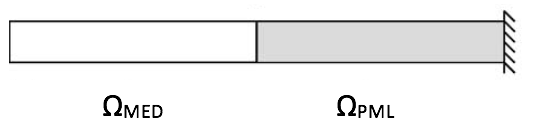
\includegraphics{images/pml_scheme.png}
    \caption{Scheme of the 2 media: on the left physical medium  and on the right the PML}
    \label{fig:sch_pml}
\end{figure}
We will impose at the extremity of the bar a force in order to create a wave. The other extremity corresponding to the end of the PML will be fixed. The algorithm will go through the following steps: 
%\begin{algorithm}[H]
% \KwData{Parameters for medium and PML}
% \KwResult{Wave propagation and absorption}
% Initialise mass, damping and stiffness matrices for  physical medium and PML \\
% Initalise displacement, velocity and acceleration vectors to 0 for medium and PML. \\
% \While{Not end time}{
%  pu_p^{n+1} \leftarrow u_p^n + h \Dot{u}_p^n + h^2(\frac{1}{2}-\beta)\Ddot{u}^n_p\\
%  p\dot{u}_p^{n+1} \leftarrow \dot{u}_p^n + h (1-\gamma)\Ddot{u}_p^n \\
%  \For{each element}{
%    Find the position of the two quadrature points \\ 
%    P_{e,int} \leftarrow \frac{c_s}{L_p} E \epsilon^n_e \left(w_1 \frac{f^p(\xi_1)}{(1+f^e(\xi_1)+ \frac{c_s h}{L_p}f^p(\xi_1))} +  w_2 \frac{f^p(\xi_2)}{(1+f^e(\xi_2)+ \frac{c_s h}{L_p}f^p(\xi_2))} \right) \\
%  }\\
%  $\Ddot{u}$_p^{n+1} \leftarrow \left[ M_p+ \gamma h C_{p} +\beta h^2 K_p  \right]^{-1}\left( P_{int} - C_p p\dot{u}^{n+1}_p - K_p pu^{n+1}_p\right)\\
%  u^{n+1}_p \leftarrow pu^{n+1}_p + h^2 \beta \Ddot{u}^{n+1}_p\\
%  $\dot{u}$^{n+1}_p \leftarrow p\dot{u}^{n+1}_p+ h \gamma \Ddot{u}^{n+1}_p\\
%  pu_m^{n+1} \leftarrow u_m^n + h \Dot{u}_m^n + h^2(\frac{1}{2}-\beta)\Ddot{u}^n_m\\
%  p\dot{u}_m^{n+1} \leftarrow \dot{u}_m^n + h (1-\gamma)\Ddot{u}_m^n \\
%  Compute the external forces applied at extremity of medium: F_{ext} \\
%  $\Ddot{u}$_m^{n+1} \leftarrow \left[ M_m+ \gamma h C_{m} +\beta h^2 K_m  \right]^{-1} \left( F_ext -  C_m p\dot{u}^{n+1}_m - K_m pu^{n+1}_m \right) \\
%  Assure the continuity of the displacement at the interface\\
%  Update displacement, velocity and acceleration for medium and PML\\
%  \For{each element}{
%  At each quadrature point
%  Calculate \epsilon^{n+1} \\
%  }\\
%  H^{n+1} \leftarrow H^n + h \epsilon^{n+1}\\
%  t\leftarrow t+h\\
% }
% \caption{Algorithm of the wave propagation from a physical medium toward the PML}
% \label{algo}
%\end{algorithm}


    


    





